
\documentclass[12pt]{mitthesis}
\usepackage{titlesec}
\usepackage{geometry}
\usepackage{graphicx}
\usepackage{booktabs, chemformula}
\usepackage{titlesec, blindtext, color}
\usepackage{listings}
\usepackage{natbib}
\usepackage{float}
\usepackage{xcolor} 
\usepackage{array}
\usepackage{color, colortbl}

\definecolor{LightCyan}{rgb}{0.93,1,1}
\newcolumntype{L}{>{\centering\arraybackslash}m{10cm}}
\newcolumntype{l}{>{\centering\arraybackslash}m{7cm}}
\def\BibTeX{{\rm B\kern-.05em{\sc i\kern-.025em b}\kern-.08em
    T\kern-.1667em\lower.7ex\hbox{E}\kern-.125emX}}

\newcommand*{\Comb}[2]{{}^{#1}C_{#2}}%

\pagestyle{plain}

\begin{document}

\title{Methods and Tools for the Analysis of Legacy Software Systems}

\author{Stana Adelina Diana}


\department{Department of Computers and Information Technology}


\thesisdate{Sept, 2019}


\supervisor{Vladimir Cretu}{Associate Professor}




\maketitle


\cleardoublepage

\setcounter{savepage}{\thepage}



\cleardoublepage



\tableofcontents

\pagestyle{plain}



\chapter{Extracting software dependencies}
\label{extraction}

\section{Tool for measuring software dependencies}
\label{sec:tool}

In order to build structural and logical dependencies we have developed a tool that takes as input the source code repository and builds the required software dependencies \cite{DepSACI}. The workflow can be delimited by three major steps as it follows (Figure \ref{fig:fig3}):\\ \\
\textit{\textbf{Step 1:} Extracting structural dependencies.}\\
\textit{\textbf{Step 2:} Extracting logical dependencies.}\\
\textit{\textbf{Step 3:} Processing the information extracted.}

\begin{figure}[H]
\centering
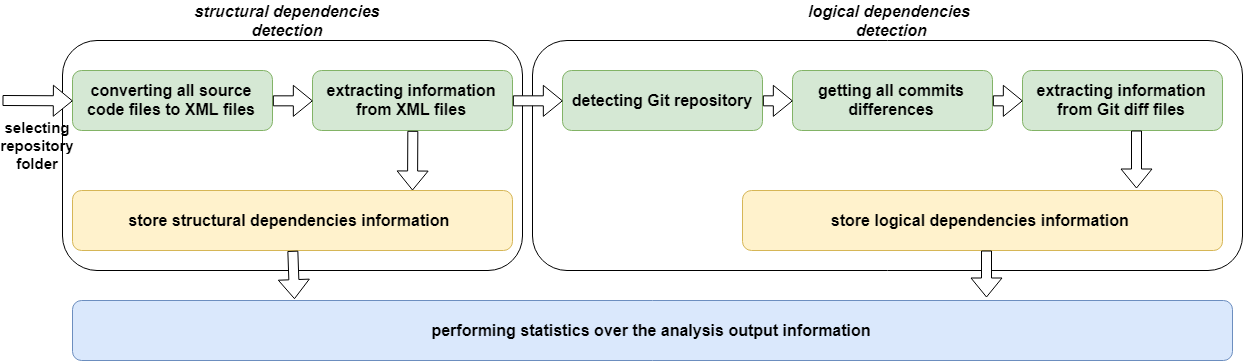
\includegraphics[width=\textwidth]{fig3.png}
\caption{Processing phases}
\label{fig:fig3}
\end{figure}


\section{Extracting structural dependencies}

A dependency is created by two elements that are in a relationship and indicates that an element of the relationship, in some manner, depends on the other element of the relationship \cite{Booch:2004:OAD:975416}, \cite{Cataldo2009SoftwareDW}.

Structural dependencies can be found by analyzing the source code \cite{Sangal:2005:UDM:1094811.1094824}, \cite{CalloArias2011}. A structural dependency between two classes A and B is given by the fact that A statically depends on B, meaning that A cannot be compiled without knowing about B. In object oriented system, this dependency can be given by many types of relationships between the two classes: A extends B, A implements B, A has attributes of type B, A has methods which have type B in their signature, A uses local variables of type B, A calls methods of B.


 We use an external tool called srcML \cite{2003:XLC:851042.857028},
\cite{Collard:2011:LTF:2067850.2068011} to convert all source code files from the current release into XML files. All the information about classes, methods, calls to other classes are afterwards extracted by our tool parsing the XML files and building a dependencies data structure. We have chosen to rely on srcML as a preprocessing tool because it reduces a significant number of syntactic differences from different programming languages and can make easier the parsing of source code written in different programming languages such as Java, C++ and C\#.    

\section{Extracting logical dependencies}

\textit{Logical dependencies} (a.k.a logical coupling) can be found by software history analysis and can reveal relationships that are not always present in the source code (structural dependencies).  

Software engineering practice has shown that sometimes modules which do not present structural dependencies still appear to be related. Co-evolution represents the phenomenon when one component changes in response to a change in another component \cite{Yu:2007:UCC:1231330.1231370}, \cite{5166450}. Those changes can be found in the software history maintained by the versioning system. Gall \cite{Gall:1998:DLC:850947.853338}, \cite{Gall:2003:CRH:942803.943741} identified as logical coupling between two modules the fact that these modules  \textit{repeatedly} change together during the historical evolution of the software system \cite{6606615}.

The versioning system contains the long-term change history of every file. Each project change made by an individual at a certain point of time is contained into a commit \cite{svn}. All the commits are stored in the versioning system chronologically and each commit has a parent. The parent commit is the baseline from which development began, the only exception to this rule is the first commit which has no parent. We will take into consideration only \textit{commits that have a parent} since the first commit can include source code files that are already in development (migration from one versioning system to another) and this can introduce redundant logical links \cite{DBLP:journals/jss/AjienkaC17}. 

The tool looks through the main branch of the project and gets all the existing commits. For each commit a diff against the parent will be made and stored. Here we have the option to ignore commits that contain more files than a threshold value for commit size. Also, we have the option to check whether the differences are in actual code or if they affect only parts of source files that are only comments.  Finally after all the difference files are stored, all the files are parsed and logical dependencies are build. For a group of files that are committed together, logical dependencies are added between all pairs formed by members of the group. Adding a logical dependency increases an occurrence counter for the logical link. \\

\chapter {Filtering extracted logical dependencies}

\section{Data set used}

We have analyzed a set of open-source projects found on GitHub\footnote{http://github.com/} \cite{Kalliamvakou2016} in order to extract the structural and logical dependencies between classes. Table \ref{table:1} enumerates all the systems studied. The 1st column assigns the projects IDs; 2nd column shows the project name; 3rd column shows the number of entities(classes and interfaces) extracted; 4th column shows the number of most recent commits analyzed from the active branch of each project and the 5th shows the language in which the project was developed.
\begin{table}[H]
\caption{Summary of open source projects studied.}
\label{table:1}
\centering
\begin{tabular}{|c|c|c|c|c|c|}
\hline
   ID  & Project    & Nr. of & Nr. of& Type\\
     &     & entites & commits & \\
\hline
1	&	bluecove	&	586	&	894	&	java	\\
2	&	aima-java	&	987	&	818	&	java	\\
3	&	powermock	&	1084	&	893	&	java	\\
4	&	restfb	&	783	&	1188	&	java	\\
5	&	rxjava	&	2673	&	2468	&	java	\\
6	&	metro-jax-ws	&	1103	&	2222	&	java	\\
7	&	mockito	&	1409	&	1572	&	java	\\
8	&	grizzly	&	1592	&	3122	&	java	\\
9	&	shipkit	&	242	&	1483	&	java	\\
10	&	OpenClinica	&	1653	&	3749	&	java	\\
11	&	robolectric	&	2050	&	5029	&	java	\\
12	&	aeron	&	541	&	5101	&	java	\\
13	&	antlr4	&	1381	&	3449	&	java	\\
14	&	mcidasv	&	805	&	3668	&	java	\\
15	&	ShareX	&	919	&	2505	&	csharp	\\
16	&	aspnetboilerplate	&	2353	&	1615	&	csharp	\\
17	&	orleans	&	3485	&	3353	&	csharp	\\
18	&	cli	&	767	&	2397	&	csharp	\\
19	&	cake	&	2250	&	1853	&	csharp	\\
20	&	Avalonia	&	1677	&	2445	&	csharp	\\
21	&	EntityFramework	&	7107	&	2443	&	csharp	\\
22	&	jellyfin	&	2179	&	4065	&	csharp	\\
23	&	PowerShell	&	861	&	2033	&	csharp	\\
24	&	WeiXinMPSDK	&	2029	&	2723	&	csharp	\\
25	&	ArchiSteamFarm	&	117	&	2181	&	csharp	\\
26	&	VisualStudio	&	1016	&	4417	&	csharp	\\
27	&	CppSharp	&	259	&	3882	&	csharp	\\
\hline
\end{tabular}
\end{table}


\section{Filtering based on the size of commit transactions}

A big commit transaction can indicate that a merge with another branch or that a renaming has been made.
In this case, a series of irrelevant logical dependencies can be introduced since not all the files are updated in the same time for a development reason. Different works have chosen fixed threshold values for the maximum number of files accepted in a commit. Cappiluppi and Ajienka, in their works \cite{DBLP:journals/jss/AjienkaC17}, \cite{DBLP:journals/ese/AjienkaCC18} only take into consideration commits with less then 10 source code files changed in building the logical dependencies.

The research of Beck et al \cite{Beck:2011:CMC:2025113.2025162} only takes in consideration transactions with up to 25 files. The research \cite{Oliva:2011:ISL:2067853.2068086} provided also a quantitative analysis of the number of files per revision; Based on the analysis of 40,518 revisions, the mean value obtained for the number of files in a revision is 6 files. However, standard deviation value shows that the dispersion is high. 

We analyzed the overall transaction size trend for 27 open-source cpp and java systems. The results are presented in Figure \ref{fig:fig_cs}, based on them we can say that 90\% of the total commit transactions made are with less than 10 source code files changed. This percent allows us to say that setting a threshold of 10 files for the maximum size of the commit transactions will not affect so much the total number of commit transactions from the systems since it will still remain 90\% of the commit transactions from where we can extract logical dependencies \cite{DepSACI}.


\begin{figure}[h]
\centering
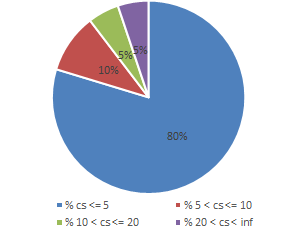
\includegraphics{fig_cs.png}
\caption{Commit transaction size(cs) trend in percentages}
\label{fig:fig_cs}
\centering
\end{figure}


\begin{figure}[h]
\centering
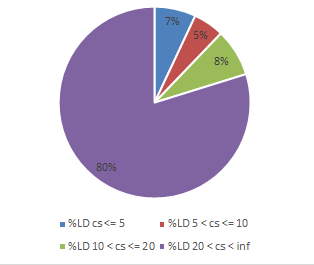
\includegraphics[scale=0.9]{fig_ld_ts.png}
\caption{Percentages of LD extracted from each commit transaction size(cs) group}
\label{fig:fig_ld_ts}
\centering
\end{figure}

As we can see in Figure \ref{fig:fig_ld_ts} even though only 5\% of the commit transactions have more than 20 files changed ($20<cs<inf$) they generate in average 80\% of the total amount of logical dependencies extracted from the systems.
The high number of logical dependencies extracted from such a small number of commit transactions is caused by big commit transactions. 
One single big commit transaction can lead to a large amount of logical dependencies. For example in RxJava we have a very few commit transactions with 1030 source code files, this means that those files can generate 
$\Comb{n}{k}=\frac{n!}{k!(n-k)!} = \frac{1030!}{2!(1028)!} = 529 935$ logical dependencies. By setting a threshold on the commit transaction size we can avoid the introduction of those logical dependencies into the system.

So filtering 10\% of the total amount of commit transactions can indeed lead to a significant decrease of the amount of logical dependencies and that is why we choose the value of 10 files as our fixed threshold for the maximum size of a commit transaction \cite{DepSACI}.



\section{Filtering based on the number of occurrences}
One occurrence of a co-change between two software entities can be a valid logical dependency, but can also be a coincidence. Taking into consideration only co-changes with multiple occurrences as valid dependencies can lead to more accurate logical dependencies and more accurate results. On the other hand, if the project studied has a relatively small amount of commits, the probability to find multiple updates of the same classes in the same time can be small, so filtering after the number of occurrences can lead to filtering all the logical dependencies extracted. Giving the fact that we will study multiple projects of different sizes and number of commits, we will analyze also the impact of this filtering on different projects.

We have performed a series of analysis on the test systems, incrementing the threshold value occ from 1 to 4. In each of the cases the extracted logical dependencies from commit transaction with less or equal to 10 changed source code files were also filtered by the minimum number of occurrences established and all the logical dependencies that did not exceeded the minimum number of occurrences were discarded. 

The results of the analysis are presented in Table \ref{table:sd_percentages} as percentages of logical dependencies (LD) that are also structural dependencies and Table \ref{table:ld_ratio} as ratio of the number of logical dependencies (LD) to the number of structural dependencies (SD).



\begin{table}[H]
\caption{Percentage of LD that are also SD}
\label{table:sd_percentages}
\centering
\begin{tabular}{|c|c|c|c|c|}
\hline
    ID  & $occ\geq 1$ & $occ\geq 2$ & $occ\geq 3$ & $occ\geq 4$  \\
\hline
1	&	7,13	&	7,77	&	7,99	&	19,71	\\
2	&	19,54	&	25,76	&	29,55	&	32,16	\\
3	&	6,66	&	8,58	&	11,82	&	14,87	\\
4	&	1,16	&	1,17	&	0,91	&	0,80	\\
5	&	3,99	&	3,96	&	7,75	&	7,49	\\
6	&	13,92	&	20,16	&	22,91	&	22,77	\\
7	&	8,38	&	9,28	&	14,93	&	14,58	\\
8	&	6,70	&	9,73	&	14,20	&	15,60	\\
9	&	16,98	&	23,34	&	29,22	&	32,89	\\
10	&	8,94	&	9,15	&	11,05	&	10,59	\\
11	&	4,99	&	6,92	&	8,88	&	11,08	\\
12	&	13,19	&	17,15	&	18,60	&	19,57	\\
13	&	2,43	&	5,59	&	8,33	&	8,21	\\
14	&	13,27	&	18,88	&	19,02	&	19,28	\\
15	&	12,90	&	21,95	&	25,51	&	27,01	\\
16	&	13,33	&	17,34	&	18,53	&	16,24	\\
17	&	6,09	&	6,18	&	6,41	&	6,44	\\
18	&	9,73	&	10,60	&	14,27	&	18,80	\\
19	&	10,26	&	13,54	&	13,64	&	12,60	\\
20	&	12,83	&	18,36	&	21,00	&	25,72	\\
21	&	2,86	&	4,65	&	5,70	&	4,98	\\
22	&	5,20	&	6,56	&	8,18	&	8,90	\\
23	&	8,23	&	13,64	&	17,04	&	17,65	\\
24	&	6,77	&	10,89	&	14,47	&	16,05	\\
25	&	9,85	&	10,15	&	11,65	&	11,33	\\
26	&	8,65	&	10,79	&	12,78	&	14,34	\\
27	&	7,04	&	8,78	&	9,87	&	10,08	\\
\hline
Avg	&	8,93	&	11,88	&	14,23	&	15,55	\\
\hline
\end{tabular}
\end{table}


\begin{table}[H]
\caption{Ratio of number of LD to number of SD}
\label{table:ld_ratio}
\centering
\begin{tabular}{|c|c|c|c|c|}
\hline
    ID  & $occ\geq 1$ & $occ\geq 2$ & $occ\geq 3$ & $occ\geq 4$  \\
\hline
1	&	4,13	&	1,94	&	1,23	&	0,26	\\
2	&	0,81	&	0,33	&	0,16	&	0,10	\\
3	&	5,12	&	1,93	&	0,78	&	0,38	\\
4	&	53,36	&	42,00	&	38,31	&	36,30	\\
5	&	4,27	&	2,90	&	0,88	&	0,72	\\
6	&	1,07	&	0,46	&	0,30	&	0,23	\\
7	&	4,09	&	2,38	&	0,99	&	0,73	\\
8	&	4,06	&	1,57	&	0,76	&	0,49	\\
9	&	3,64	&	2,03	&	1,14	&	0,77	\\
10	&	1,41	&	1,01	&	0,47	&	0,34	\\
11	&	7,91	&	4,47	&	2,93	&	2,03	\\
12	&	3,92	&	2,15	&	1,47	&	1,07	\\
13	&	10,15	&	3,18	&	1,22	&	1,03	\\
14	&	3,07	&	1,53	&	1,16	&	0,97	\\
15	&	2,34	&	0,84	&	0,48	&	0,33	\\
16	&	1,21	&	0,47	&	0,26	&	0,19	\\
17	&	2,99	&	1,83	&	1,11	&	0,84	\\
18	&	2,26	&	1,37	&	0,67	&	0,40	\\
19	&	2,32	&	1,38	&	0,76	&	0,67	\\
20	&	1,24	&	0,58	&	0,35	&	0,18	\\
21	&	5,33	&	2,12	&	1,27	&	1,05	\\
22	&	3,38	&	1,88	&	0,99	&	0,74	\\
23	&	3,62	&	1,22	&	0,76	&	0,37	\\
24	&	2,57	&	1,22	&	0,67	&	0,46	\\
25	&	7,47	&	5,36	&	4,16	&	3,73	\\
26	&	4,03	&	2,16	&	1,50	&	1,15	\\
27	&	7,46	&	4,26	&	2,99	&	2,43	\\
\hline
Avg	&	5,67	&	3,43	&	2,51	&	2,15	\\
\hline
\end{tabular}
\end{table}




Based on Table \ref{table:sd_percentages} we can say that only a small percentage of the extracted logical dependencies are also structural dependencies. This is consistent with the findings of related works \cite{DBLP:journals/jss/AjienkaC17}, \cite{DBLP:journals/ese/AjienkaCC18}. The percentage of LD which are also SD  increases with the minimum number of occurrences because the number of logical dependencies from the systems decreases with the minimum number of occurrences. 
We calculate the overlapping between logical and structural dependencies not only because we want to get an idea of how many structural dependencies are reflected in the versioning system through logical dependencies but also because we want to eliminate logical dependencies that are also structural dependencies since they don't bring any new information to the systems.

We stopped the minimum occurrences threshold to 4 because we observed that for systems with ID 2, 6, 10 and 16 from Table \ref{table:ld_ratio} the ratio number is lower than 1 which means that the number of SD is higher than the number of LD. On the other hand for systems with ID 4, 11, 25, 27 the threshold of 4 for minimum number of occurrences does not change the discrepancy between the number of logical and structural dependencies.
If we try to go higher with the occurrences threshold we will risk to filter all the existing logical dependencies for some of the systems.
So, filtering with a threshold of 4 for the minimum number of occurrences will indeed filter the logical dependencies but for some of the systems the remaining number of logical dependencies will still be significantly higher compared to the number of structural dependencies.



\section{Overlaps between structural and logical dependencies}
A logical dependency can be also a structural dependency and vice-versa, so studying the overlapping between logical and structural dependencies while filtering is important since the intention is to introduce those logical dependencies among with structural dependencies in architectural reconstruction systems. Current studies have shown a relatively small percentage of overlapping between them with and without any kind of filtering \cite{DBLP:journals/jss/AjienkaC17}. This means that a lot of non related entities update together in the versioning system, the goal here is to establish the factors that determine such a small percentage of overlapping \cite{enase19}.


In the main series of experiments, for each system, we extracted the structural dependencies and the logical dependencies and determined the overlap between the two dependencies sets, in various experimental conditions. 

One variable experimental condition is whether changes located in comments contribute towards logical dependencies. This condition distinguishes between two different cases: 
\begin{itemize}
	\item with comments: a change in source code files is counted towards a logical dependency, even if the change is inside comments in all files
	\item without comments: commits that changed source code files only by editing comments are ignored as logical dependencies
\end{itemize}

In all cases, we varied the following threshold values: 
 \begin{itemize}
	\item commit size ($cs$): the maximum size of commit transactions which are accepted to generate logical dependencies. The values for this threshold were 5, 10, 20 and no threshold (infinity).  
	\item number of occurrences ($occ$): the minimum number of repeated occurrences for a co-change to be counted as logical dependency. The values for this threshold were 1, 2, 3 and 4.  
\end{itemize}

The six tables below present the synthesis of our experiments. 
We have computed the following  values:
\begin{itemize}
	\item the mean ratio of the number of logical dependencies  (LD) to the number of structural dependencies (SD)
   \item the mean percentage of structural dependencies that are also logical dependencies (calculated from the number of overlaps divided to the number of structural dependencies)	
		\item the mean percentage of logical dependencies that are also structural dependencies (calculated from the number of overlaps divided to the number of logical dependencies)
\end{itemize}

In all the six tables, \ref{tab:ratio:comm}, \ref{tab:ratio:nocomm}, \ref{tab:percSD:comm}, \ref{tab:percSD:nocomm},
\ref{tab:percLD:comm}, \ref{tab:percLD:nocomm} we have on columns the values used for the commit size $cs$, while on rows we have the values for the number of occurrences threshold $occ$. The tables contain median values obtained for experiments done under all combinations of the two threshold values, on all test systems. In all tables, the upper right corner corresponds to the most relaxed filtering conditions, while the lower left corner corresponds to the most restrictive filtering conditions.

\begin{table}[!h]
%% increase table row spacing, adjust to taste
\renewcommand{\arraystretch}{1}
\caption{Ratio of number of LD to number of SD, case with comments}
\label{tab:ratio:comm}
\centering

\begin{tabular}{|c|c|c|c|c|}
\hline
	      &	$cs\leq 5$	&	$cs\leq 10$	&	$cs\leq 20$	&	$cs<\infty$	\\
\hline
$occ\geq 1$	&	3,39	&	5,67	&	9,00	&	80,31	\\
$occ\geq 2$	&	2,24	&	3,47	&	5,02	&	60,14	\\
$occ\geq 3$	&	1,04	&	2,53	&	3,52	&	44,68	\\
$occ\geq 4$	&	0,90	&	2,16	&	2,88	&	33,47	\\
\hline
\end{tabular}
\end{table}

\begin{table}[!h]
%% increase table row spacing, adjust to taste
\renewcommand{\arraystretch}{1}
\caption{Ratio of number of LD to number of SD, case without comments}
\label{tab:ratio:nocomm}
\centering

\begin{tabular}{|c|c|c|c|c|}
\hline
	      &	$cs\leq 5$	&	$cs\leq 10$	&	$cs\leq 20$	&	$cs< \infty$	\\
\hline
$occ\geq 1$	&	3,24	&	5,33	&	7,90	&	67,16	\\
$occ\geq 2$	&	1,35	&	3,27	&	4,72	&	47,39	\\
$occ\geq 3$	&	1,00	&	1,67	&	2,49	&	32,39	\\
$occ\geq 4$	&	0,43	&	1,26	&	1,93	&	22,15	\\
\hline
\end{tabular}
\end{table}

\begin{table}[!h]
%% increase table row spacing, adjust to taste
\renewcommand{\arraystretch}{1}
\caption{Percentage of SD that are also LD, case with comments}
\label{tab:percSD:comm}
\centering

\begin{tabular}{|c|c|c|c|c|}
\hline
	      &	$cs\leq 5$	&	$cs\leq 10$	&	$cs\leq 20$	&	$cs< \infty$	\\
\hline
$occ\geq 1$	&	19,75	&	29,86	&	39,29	&	76,59	\\
$occ\geq 2$	&	12,50	&	20,20	&	27,68	&	66,11	\\
$occ\geq 3$	&	8,49	&	14,22	&	19,94	&	55,99	\\
$occ\geq 4$	&	6,58	&	10,95	&	15,76	&	47,12	\\
\hline
\end{tabular}
\end{table}

\begin{table}[!h]
%% increase table row spacing, adjust to taste
\renewcommand{\arraystretch}{1}
\caption{Percentage of SD that are also LD, case without comments}
\label{tab:percSD:nocomm}
\centering

\begin{tabular}{|c|c|c|c|c|}
\hline
	      &	$cs\leq 5$	&	$cs\leq 10$	&	$cs\leq 20$	&	$cs< \infty$	\\
\hline
$occ\geq 1$	&	18,88	&	28,47	&	37,44	&	71,12	\\
$occ\geq 2$	&	11,87	&	19,03	&	25,93	&	59,58	\\
$occ\geq 3$	&	8,00	&	13,09	&	18,15	&	48,65	\\
$occ\geq 4$	&	5,85	&	9,94	&	14,27	&	39,07	\\
\hline
\end{tabular}
\end{table}

\begin{table}[!h]
%% increase table row spacing, adjust to taste
\renewcommand{\arraystretch}{1}
\caption{Percentage of LD that are also SD, case with comments}
\label{tab:percLD:comm}
\centering

\begin{tabular}{|c|c|c|c|c|}
\hline
	      &	$cs\leq 5$	&	$cs\leq 10$	&	$cs\leq 20$	&	$cs< \infty$	\\
\hline
$occ\geq 1$	&	12,02	&	8,86	&	6,72	&	1,79	\\
$occ\geq 2$	&	15,05	&	11,71	&	9,38	&	2,21	\\
$occ\geq 3$	&	17,45	&	13,97	&	11,57	&	2,86	\\
$occ\geq 4$	&	18,96	&	15,28	&	12,94	&	3,67	\\
\hline
\end{tabular}
\end{table}

\begin{table}[!h]
%% increase table row spacing, adjust to taste
\renewcommand{\arraystretch}{1}
\caption{Percentage of LD that are also SD, case without comments}
\label{tab:percLD:nocomm}
\centering
\begin{tabular}{|c|c|c|c|c|}
\hline
	      &	$cs\leq 5$	&	$cs\leq 10$	&	$cs\leq 20$	&	$cs< \infty$	\\
\hline
$occ\geq 1$	&	12,05	&	9,02	&	6,98	&	1,93	\\
$occ\geq 2$	&	15,08	&	12,03	&	9,66	&	2,42	\\
$occ\geq 3$	&	17,78	&	14,37	&	12,24	&	3,28	\\
$occ\geq 4$	&	19,22	&	15,59	&	13,30	&	4,21	\\
\hline
\end{tabular}
\end{table}

In order to assess the influence of comments, we compare pairwise Tables \ref{tab:ratio:comm} and \ref{tab:ratio:nocomm},  
Tables \ref{tab:percSD:comm} and \ref{tab:percSD:nocomm} and Tables \ref{tab:percLD:comm} and \ref{tab:percLD:nocomm}. 
We observe that, although there are some differences between pairs of measurements done in similar conditions with and without comments, the differences are not significant.

On the other hand, the overlap between structural and logical dependencies is given by the number of pairs of classes that have both structural and logical dependencies. We evaluate this overlap as a percentage relative to the number of structural dependencies in Tables \ref{tab:percSD:comm} and \ref{tab:percSD:nocomm}, respectively as  a percentage relative to the number of logical dependencies in Tables \ref{tab:percLD:comm} and \ref{tab:percLD:nocomm}.

A first observation from Tables \ref{tab:percSD:comm} and \ref{tab:percSD:nocomm} is that not all pairs of classes with structural dependencies co-change. The biggest value for the percentage of structural dependencies that are also logical dependencies is 76.5\% obtained in the case when no filterings are done.

From Tables \ref{tab:percLD:comm} and \ref{tab:percLD:nocomm} we notice that the percentage of logical dependencies which are also structural is always low to very low. This means that most co-changes are recorded between classes that have no structural dependencies to each other \cite{enase19}.   
 
\chapter{Usage of the extracted dependencies}
\section{Data set used}
To extract the key classes based on logical dependencies, we took the same set of data used in another research involving key class detection. The research of I. Sora et al \cite{Finding-key-classes} takes into consideration structural public dependencies that are extracted using static analysis techniques and was performed on the object-oriented systems presented in table \ref{tab:keyclass:overview}.

The requirements for a system to qualify as suited for investigations using logical dependencies are: has to be on GitHub, has to have release tags to identify the version, and also has to have an increased number of commits. 
From the total of 14 object-oriented systems listed in the paper \cite{Finding-key-classes}, 13 of them have repositories in Github \ref{tab:gitfoundsystems}. And from the found repositories we identified only 6 repositories that have the same release tag as the specified version from table \ref{tab:keyclass:overview}. It is important to identify the correct release tag for each repository to limit the commits further analyzed by date. Only commits that were made until the specified release are considered and analyzed.
The commits number found on the remaining 6 repositories varies from 19108 commits for Tomcat Catalina to 149 commits for JHotDraw. In order to have more accurate results, we need a significant number of commits, so we reached the conclusion that only 3 systems can be used for key classes detection using logical dependencies: Apache Ant, Hibernate, and Tomcat Catalina.  From all the systems mentioned in table \ref{tab:keyclass:overview} Apache Ant is the most used and analyzed in other  works \cite{enase19}, \cite{7332515}, \cite{1402122}, \cite{Kamran2016IdentificationOC}.

\begin{table}[H]
\renewcommand{\arraystretch}{1}
\caption{Analyzed software systems in previous research paper.}
\label{tab:keyclass:overview}
\centering
\begin{tabular}{|c|c|L|c|}
\hline
ID	&	System	&	Description	&	Version	\\
\hline
Sl	&	Apache Ant	&	Java library and command line tool that drive the build processes as targets and extension points depending upon each other	&	1.6.1	\\
S2	&	Argo UML	&	UML modelling tool with support for all UML diagrams.	&	0.9.5	\\
S3	&	GWT Portlets	&	Open source web framework for building GWT (Google Web Toolkit) Applications.	&	0.9.5 beta	\\
S4	&	Hibernate 	&	Persistence framework for Java.	&	5.2.12	\\
S5	&	javaclient	&	Java distributed application for playing with robots	&	2.0.0	\\
S6	&	jEdit	&	Java mature text editor for programmers.	&	5.1.0	\\
S7	&	JGAP	&	Genetic Algorithms and Genetic Programming Java library.	&	3.6.3	\\
S8	&	JHotDraw	&	JHotDraw is a two-dimensional graphics framework for structured drawing editors that is written in Java.	&	6.0b.1	\\
S9	&	JMeter	&	JMeter is a Java application designed to load test functional behavior and measure performance	&	2.0.1	\\
S10	&	Log4j	&	Logging Service	&	2.10.0	\\
S11	&	Mars	&	The Mars Simulation Project is a Java project that models and simulates human settlements on Mars planet	&	3.06.0	\\
S12	&	Maze	&	The Maze-solver project simulates an artificial intelligence algorithm on a maze	&	1.0.0	\\
S13	&	Neuroph	&	Neuroph is a Java neural network framework.	&	2.2.0	\\
S14	&	Tomcat Catalina	&	The Apache Tomcat project is an open-source implementation of JavaServlet and JavaServerPages technologies	&	9.0.4	\\
S15	&	Wro4J	&	The Wro4J is a web resource (JS and CSS) optimizer for Java.	&	1.6.3	\\
\hline
\end{tabular}
\end{table}



\begin{table}[H]
\renewcommand{\arraystretch}{1}
\caption{Found systems and versions of the systems in GitHub. }
\label{tab:gitfoundsystems}
\centering
\begin{tabular}{|c|c|c|c|c|}
\hline
ID	&	System	&	Version	&	Release Tag name	&	Commits number	\\
\hline
\rowcolor{LightCyan}
Sl	&	Apache Ant	&	1.6.1	&	rel/1.6.1	&	6713	\\
S2	&	Argo UML	&	0.9.5	&	not found	&	0	\\
S3	&	GWT Portlets	&	0.9.5 beta	&	not found	&	0	\\
\rowcolor{LightCyan}
S4	&	Hibernate 	&	5.2.12	&	5.2.12	&	6733	\\
S5	&	javaclient	&	2.0.0	&	not found	&	0	\\
S6	&	jEdit	&	5.1.0	&	not found	&	0	\\
S7	&	JGAP	&	3.6.3	&	not found	&	0	\\
S8	&	JHotDraw	&	6.0b.1	&	not found	&	149	\\
S9	&	JMeter	&	2.0.1	&	v2\_1\_1	&	2506	\\
S10	&	Log4j	&	2.10.0	&	v1\_2\_10-recalled	&	634	\\
S11	&	Mars	&	3.06.0	&	not found	&	0	\\
S12	&	Maze	&	1.0.0	&	not found	&	0	\\
S13	&	Neuroph	&	2.2.0	&	not found	&	0	\\
\rowcolor{LightCyan}
S14	&	Tomcat Catalina	&	9.0.4	&	9.0.4	&	19108	\\
S15	&	Wro4J	&	1.6.3	&	v1.6.3	&	2871	\\

\hline
\end{tabular}
\end{table}


\section{Identifying key classes using logical dependencies}
\subsection{Definition and previous work}
Zaidman et al \cite{ZaidmanJurnal} were the first to introduce the concept of key classes and it refers to classes that can be found in documents written to provide an architectural overview of the system or an introduction to the system structure. 
Tahvildari and Kontogiannis have a more detailed definition regarding key classes concept: “Usually, the most important concepts of a system are implemented by very few key classes which can be characterized by the specific properties. These classes, which we refer to as key classes, manage many other classes or use them in order to implement their functionality. The key classes are tightly coupled with other parts of the system. Additionally, they tend to be rather complex, since they implement much of the legacy system’s functionality” \cite{Tahvildari2004ImprovingDQ}.
Also, other researchers use a similar concept as the one defined by Zaidman but under different terms like important classes  \cite{Meyer2014IdentifyingIC} or central software classes \cite{CentralClassesSteidl}.


In previous works, the approach for finding key classes is based on ranking the classes with a page ranking algorithm \cite{PagerankENASE}, \cite{enase15}, \cite{Finding-key-classes}, \cite{PagerankSACI} . The page ranking algorithm is a customization of PageRank, the algorithm used to rank web pages \cite{ilprints422}. 
The PageRank algorithm works based on a recommendation system. If one node has a connection with another node, then it recommends the second node. In previous works, connections are established based on structural dependencies extracted from static code analysis. If A has a structural dependency with B, then A recommends B, and also B recommends A. 

\subsection{Metrics to determine key classes}
In order to identify the key classes of an object-oriented system, we have to determine what metrics can be used in order to get a good overview of the system and its most important classes \cite{Ding2016AnIA}, \cite{ZaidmanJurnal}, \cite{PAN2018188} . 
The metrics used in previous research can be grouped into the following categories: 

\begin{itemize}
	\item class size metrics: number of fields (NoF),  number of methods (NoM), global size (Size = NoF+NoM).
	\item class connection metrics, any structural dependency between two classes:
		\begin{itemize}
			\item CONN-IN, the number of distinct classes that use a class;
			\item CONN-OUT, the total number of distinct classes that are used by a class;
			\item CONN-TOTAL, the total number of distinct classes that a class uses or are used by a class (CONN-IN + CONN-OUT).
			\item CONN-IN-W, the total weight of distinct classes that use a class. 
			\item CONN-OUT-W, the total weight of distinct classes that are used by a class. 
			\item CONN-TOTAL-W, the total weight of all connections of the class (CONN-IN-W + CONN-OUT-W) \cite{Finding-key-classes}.
		\end{itemize}
	\item class pagerank values, previous research use pagerank values computed on both directed and undirected, weighted and unweighted graphs:
		\begin{itemize}
			\item PR - value computed on the directed and unweighted graph;
			\item PR-W - value computed on the directed and weighted graph;
			\item PR-U - value computed on the undirected and unweighted graph;
			\item PR-U-W - value computed on the undirected and weighted graph;
			\item PR-U2-W - value computed on the weighted graph with back-recommendations \cite{PagerankENASE}, \cite{enase15}, \cite{Finding-key-classes}, \cite{PagerankSACI}.
		\end{itemize}
\end{itemize}

\subsection{Measurements}

\begin{table}[!h]
\renewcommand{\arraystretch}{1}
\caption{Measurements for Ant}
\label{tab:measurements:ant}
\centering
\begin{tabular}{|c|ccccccccccc|}
\hline
 &	10	&	20	&	30	&	40	&	50	&	60	&	70	&	80	&	90	&	100	&	Previous \\
\hline
PR\_U2\_W	&	0.70	&	0.64	&	0.75	&	0.66	&	0.63	&	0.75	&	0.81	&	\cellcolor{LightCyan}0.87	&	0.79	&	0.79	&	0.93	\\							
PR	&	0.70	&	0.64	&	0.75	&	0.66	&	0.63	&	0.75	&	0.81	&	\cellcolor{LightCyan}0.87	&	0.79	&	0.79	&	0.86	\\							
PR\_U	&	0.70	&	0.64	&	0.75	&	0.66	&	0.63	&	0.75	&	0.81	&	\cellcolor{LightCyan}0.87	&	0.79	&	0.79	&	0.93	\\							
CONN\_TOTAL\_W	&	0.73	&	0.70	&	0.67	&	0.66	&	0.65	&	0.73	&	0.80	&	\cellcolor{LightCyan}0.84	&	0.80	&	0.80	&	0.93	\\							
CONN\_TOTAL	&	0.73	&	0.70	&	0.67	&	0.66	&	0.65	&	0.73	&	0.80	&	\cellcolor{LightCyan}0.84	&	0.80	&	0.80	&	0.94	\\							

\hline
\end{tabular}
\end{table}

\begin{table}[!h]
\renewcommand{\arraystretch}{1}
\caption{Measurements for Hibernate}
\label{tab:measurements:hibernate}
\centering
\begin{tabular}{|c|ccccccc|}
\hline
 &	50	&	60	&	70	&	80	&	90	&	100	&	Previous \\
\hline
PR\_U2\_W	&	0.61	&	0.64	&	0.65	&	0.66	&	0.66	&	\cellcolor{LightCyan}0.66	&	0.96	\\
PR	&	0.61	&	0.64	&	0.65	&	0.66	&	0.66	&	\cellcolor{LightCyan}0.66	&	0.95	\\
PR\_U	&	0.61	&	0.64	&	0.65	&	0.66	&	0.66	&	\cellcolor{LightCyan}0.66	&	0.95	\\
CONN\_TOTAL\_W	&	0.61	&	0.64	&	0.65	&	0.66	&	0.66	&	\cellcolor{LightCyan}0.66	&	0.94	\\
CONN\_TOTAL	&	0.61	&	0.64	&	0.65	&	0.66	&	0.66	&	\cellcolor{LightCyan}0.66	&	0.95	\\
\hline
\end{tabular}
\end{table}


\begin{table}[!h]
\renewcommand{\arraystretch}{1}
\caption{Measurements for Tomcat Catalina}
\label{tab:measurements:tomcat}
\centering
\begin{tabular}{|c|ccccccccccc|}
\hline
 &	10	&	20	&	30	&	40	&	50	&	60	&	70	&	80	&	90	&	100	&	Previous \\
\hline
PR\_U2\_W	&	0.70	&	0.63	&	0.63	&	0.71	&	0.74	&	0.77	&	0.79	&	\cellcolor{LightCyan}0.80	&	0.80	&	0.80	&	0.92	\\							
PR	&	0.67	&	0.62	&	0.63	&	0.71	&	0.74	&	0.77	&	0.79	&	\cellcolor{LightCyan}0.80	&	0.80	&	0.80	&	0.93	\\							
PR\_U	&	0.67	&	0.62	&	0.63	&	0.71	&	0.74	&	0.77	&	0.79	&	\cellcolor{LightCyan}0.80	&	0.80	&	0.80	&	0.93	\\							
CONN\_TOTAL\_W	&	0.68	&	0.60	&	0.62	&	0.71	&	0.74	&	0.77	&	0.79	&	\cellcolor{LightCyan}0.80	&	0.80	&	0.80	&	0.93	\\							
CONN\_TOTAL	&	0.64	&	0.59	&	0.62	&	0.71	&	0.74	&	0.77	&	0.79	&	\cellcolor{LightCyan}0.80	&	0.80	&	0.80	&	0.94	\\							
\hline
\end{tabular}
\end{table}

\section{Comparison of the extracted data with FAN-IN and FAN-OUT metric}


 %%%%%%%%%%%%%%%%%%%%%%%%%%%%%%%%%%%%%%%%%%%%%%%%%%%%%%%%%%%%%%%%%%%%%%%%%%%%%%%%


\bibliographystyle{plain}
\bibliography{logicaldepd}
\end{document}

